\section{研究方法}

%%%%%%%%%%%%%%%%%%%%%%%%%%%%%%
\subsection{理论模型:分布共享数据}

%%%%%%%%%%%%%%%
\begin{frame}{分布共享数据 (I)}
  \fig{width = 0.40\textwidth}{figures/dsm4replicas-model.pdf}{分布数据共享服务.}
\end{frame}
%%%%%%%%%%%%%%%
\begin{frame}{分布共享数据 (II)}
  \begin{center}
    \textcolor{cyan}{$x, y:$} 共享变量 \hspace{0.30cm} \textcolor{cyan}{$p_0, p_1:$} 
    客户进程
  \end{center}

  多进程并发提交 (读/写) 操作:
  
  \fignocaption{width = 0.55\textwidth}{figures/register-what-value.pdf}

  \begin{center}
    \question{问题: 读操作允许返回什么值?}
  \end{center}

  \answer{
  \[
    \text{不同一致性}
    \xrightleftharpoons[\text{定义}]{\,\text{规定}\,}
    \text{不同合法返回值}
  \]} 
\end{frame}
%%%%%%%%%%%%%%%
\begin{frame}{分布共享数据 (III)}
  \begin{center}
    \textcolor{blue}{\large 基本定位: 传统概念应用于新型平台}
  \end{center}

  \vspace{0.20cm}
  \begin{center}
    分布共享数据服务: 分布共享内存模型 + 分布数据系统
  \end{center}
\end{frame}
%%%%%%%%%%%%%%%
\begin{frame}{分布共享内存 (I)}
  \begin{figure}
    \begin{subfigure}{0.50\linewidth}
      \centering
      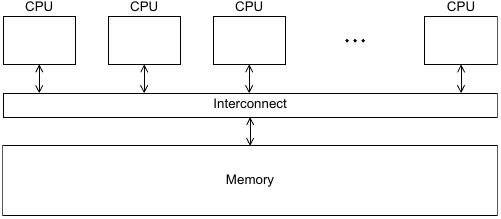
\includegraphics[width=0.80\textwidth]{figures/shared-memory.png}
      \caption{共享内存系统.}
    \end{subfigure}%
    \begin{subfigure}{0.50\linewidth}
      \centering
      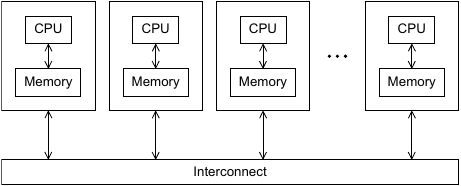
\includegraphics[width=0.85\textwidth]{figures/distributed-memory.png}
      \caption{分布内存系统.}
    \end{subfigure}
    \caption{多处理器系统体系结构 \todo{重绘}.}
  \end{figure}
\end{frame}
%%%%%%%%%%%%%%%
\begin{frame}{分布共享内存 (II)}
  分布内存系统实例: 按系统耦合度分类
\end{frame}
%%%%%%%%%%%%%%%
\begin{frame}{分布共享内存 (III)}
  \begin{center}
    分布共享内存: 在\textcolor{blue}{分布内存}之上提供\textcolor{blue}{共享内存}的假象
  \end{center}

  \todo{图: 分布共享内存 (from Kai Li)}
\end{frame}
%%%%%%%%%%%%%%%
\begin{frame}{分布共享数据 (IV)}
  问题空间: 传统问题, 新平台, 新挑战 (\todo{总结})

  目的: 并行编程

  实现手段: 硬件/操作系统

  
\end{frame}
%%%%%%%%%%%%%%%%%%%%%%%%%%%%%%
\subsection{技术途径: 三维框架}

%%%%%%%%%%%%%%%
\begin{frame}{分布共享内存中的数据一致性问题}
      数据一致性问题的三个层面: 
      \begin{description}
	\item[1. 虚拟共享数据有什么?]
	  \begin{itemize}
	    \item 数据类型
	  \end{itemize}
	\item[2. 上层接口语义是什么?]
	  \begin{itemize}
	    \item 一致性模型
	  \end{itemize}
	\item[3. 底层消息传递为什么?]
	  \begin{itemize}
	    \item 一致性保障
	  \end{itemize}
      \end{description}
\end{frame}
%%%%%%%%%%%%%%%
\begin{frame}{研究框架}
  \fig{width = 0.75\textwidth}{figures/thesis-proposal-3d-framework-allinone.pdf}{数据一致性及保障技术研究框架}
\end{frame}
%%%%%%%%%%%%%%%
\begin{frame}{研究挑战}
  \fignocaption{width = 0.40\textwidth}{figures/sla.jpg}

  用户对一致性的需求:
  \begin{enumerate}
    \setlength{\itemsep}{5pt}
    \item 多样化, 可定制 \citeinbeamer{Terry}{CACM}{13}
    \uncover<2->{
      \begin{description}
        \item[多样化:] 
          \begin{itemize}
            \item 一致性族: causality; read-your-writes {\scriptsize (RYW)}
            \item 参数调节: 提供``有限度''的不一致 \citeinbeamer{Yu}{TOCS}{02}
          \end{itemize}
        \item[可定制:] 混合使用, 运行时可变
      \end{description}
    }
  \item 精细化, 可度量 \citeinbeamer{Bailis}{VLDB}{12}
    \uncover<3->{
      \begin{description}
        \item[精细化:] ``在大多数情况下, 访问到一致数据''
        \item[可度量:] 量化系统执行, 后验系统对一致性的满足程度 
      \end{description}
    }
  \end{enumerate}
\end{frame}
